\documentclass{article}

\usepackage[utf8]{inputenc}
\usepackage[spanish,es-lcroman]{babel}
\usepackage{fancyhdr}
\usepackage{lastpage}
\usepackage{extramarks}
\usepackage[usenames,dvipsnames]{color}
\usepackage{graphicx}
\usepackage{listings}
\usepackage{xparse}
\usepackage{courier}
\usepackage{amsmath}
\usepackage{enumitem}
\usepackage{hyperref}
\hypersetup{
    colorlinks=true,
    linkcolor=blue,
    urlcolor=blue,
    linktoc=all
}

\setenumerate[1]{label=(\alph*)}

% Margenes
\topmargin=-0.65in
\evensidemargin=0in
\oddsidemargin=0in
\textwidth=6.5in
\textheight=9.0in
\headsep=0.25in

% Header y footer
\pagestyle{fancy}
\lhead{}
\chead{\tareaRamo\ (\tareaProfesor): \tareaTitulo} % Centro
\rhead{\firstxmark}
\lfoot{\lastxmark}
\cfoot{}
\rfoot{Página\ \thepage\ de\ \protect\pageref{LastPage}} % Pagina
\renewcommand\headrulewidth{0.4pt}
\renewcommand\footrulewidth{0.4pt}

\setlength\parindent{0pt} % Eliminar la indentación

\newcommand{\python}[2]{
\begin{itemize}
\item[]\lstinputlisting[language=Python,caption=#2,label=#1]{#1.py}
\end{itemize}
}

%----------------------------------------------------------------------------------------
%	Meta Información
%----------------------------------------------------------------------------------------
\newcommand{\tareaTitulo}{Tarea\ \#3 - Informe} % titulo del informe
\newcommand{\tareaFecha}{\today} % Fecha
\newcommand{\tareaRamo}{Redes de Computadores} % Ramo
\newcommand{\tareaUniversidad}{Departamento\ de\ Informática\ UTFSM, Santiago} %usm
\newcommand{\tareaProfesor}{Oscar\ Encina} % Profesor
\newcommand{\tareaAyudante}{Alex\ Arenas} % Ayudante
\newcommand{\tareaAlumnoUno}{Eduardo\ Fernandez\ S.} % Nombre Alumno 1
\newcommand{\tareaAlumnoDos}{Victor Cifuentes S.} % Nombre Alumno 2
\newcommand{\tareaRolUno}{2010-} % Rut alumno 1
\newcommand{\tareaRolDos}{201073557-5} % Rut Alumno 2

%----------------------------------------------------------------------------------------
%	Título
%----------------------------------------------------------------------------------------

\title{
\textmd{\textbf{\tareaRamo:\ \tareaTitulo}}\\
\normalsize\vspace{0.1in}\small{\tareaFecha}\\
\vspace{0.1in}\large{Profesor: \textit{\tareaProfesor} \qquad \qquad Ayudante: \textit{\tareaAyudante}}
}

\author{
    \textbf{\tareaAlumnoUno} \\
    \small{\tareaRolUno}
    \and
    \textbf{\tareaAlumnoDos} \\
    \small{\tareaRolDos}}
\date{}

%----------------------------------------------------------------------------------------

\begin{document}

\maketitle

\section{Pregunta 1}	

En esta secci\'on se analizar\'an 5 direcciones donde se describir\'a el viaje de los paquetes y las rutas que toman.

Usando $Open Visual Tracerouter$ se obtienen las siguientes im\'agenes para cada direcci\'on:

\begin{itemize}
\item http://moodle.inf.utfsm.cl\\

\begin{center}$
\begin{array}{c}
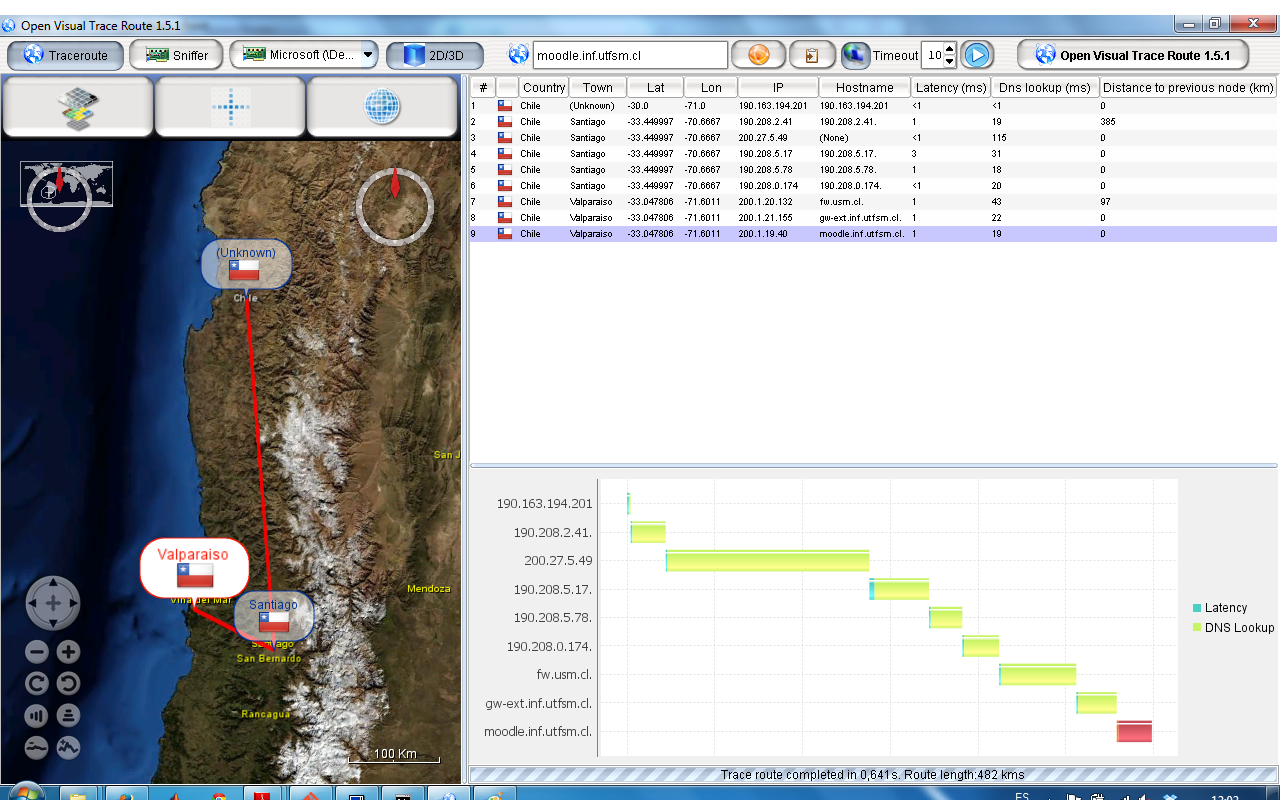
\includegraphics[width=6in]{Redes_moodle_TR.png}
\end{array}$
\end{center}

\item http://google.cl\\

\begin{center}$
\begin{array}{c}
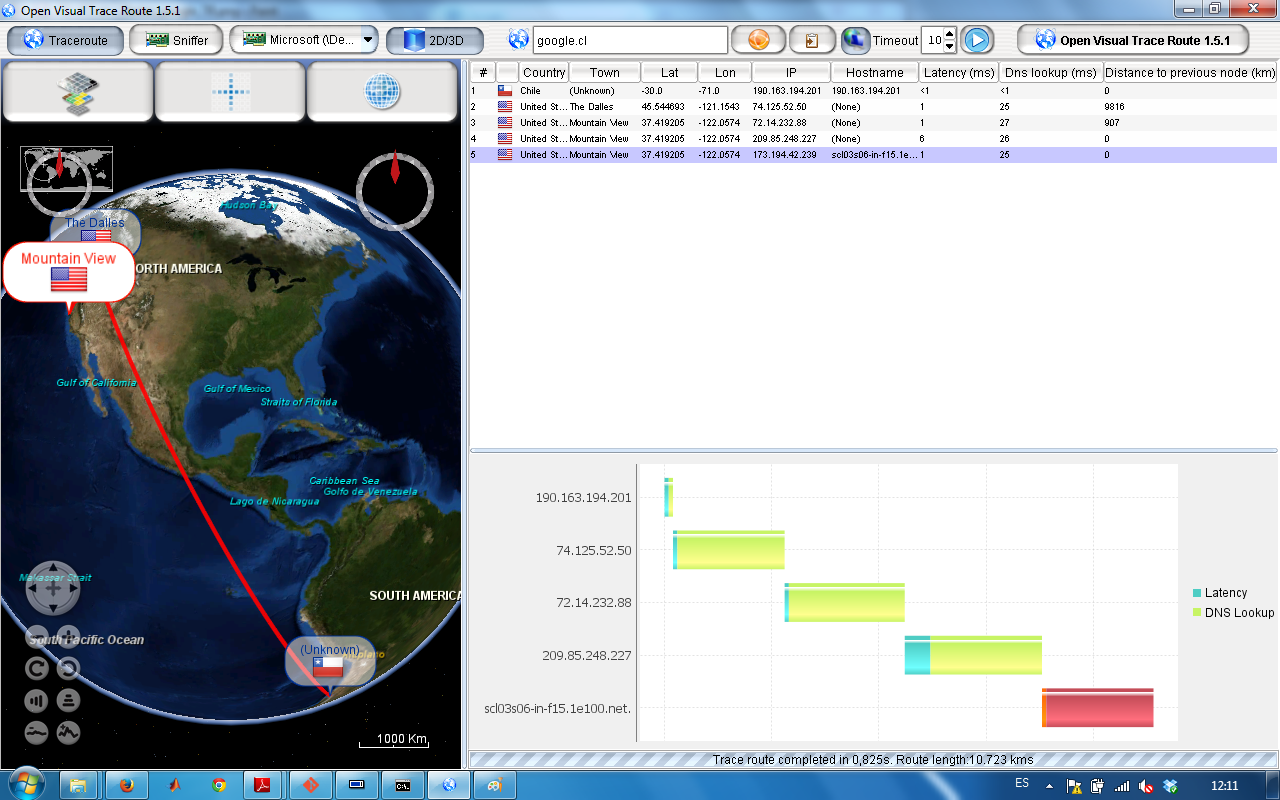
\includegraphics[width=6in]{Redes_google_TR.png}
\end{array}$
\end{center}

\item http://cime.cl\\

\begin{center}$
\begin{array}{c}
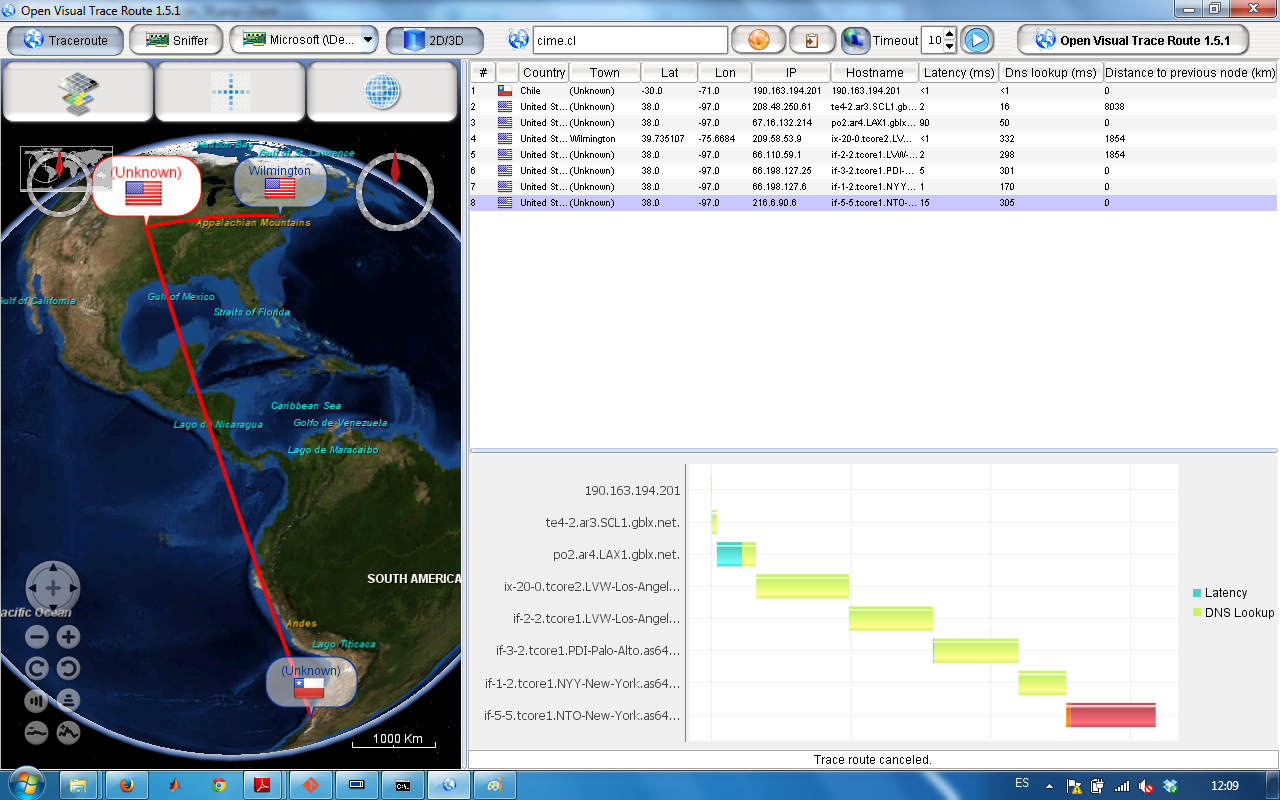
\includegraphics[width=6in]{Redes_cime_TR.png}
\end{array}$
\end{center}

\item http://wikipedia.com\\

\begin{center}$
\begin{array}{c}
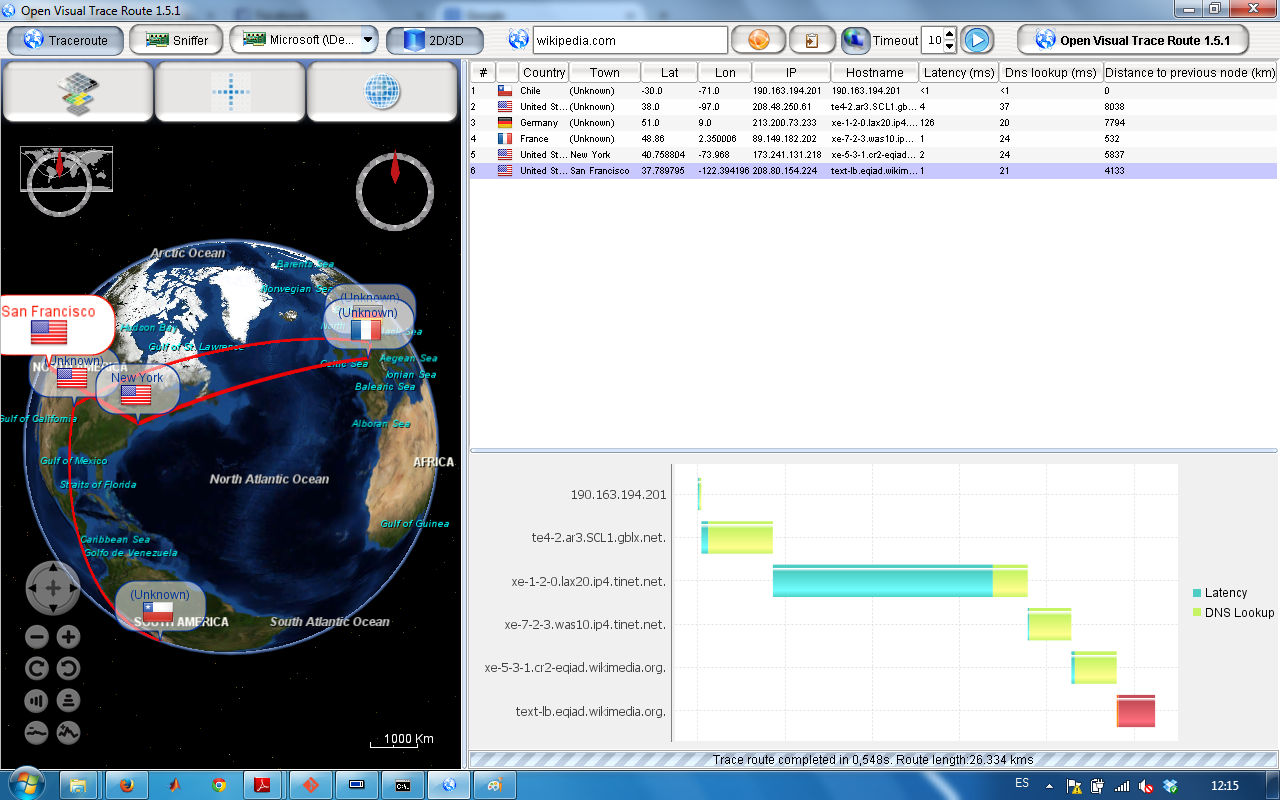
\includegraphics[width=6in]{Redes_wikipedia_TR.png}
\end{array}$
\end{center}

\item http://www.chile.embassy.gov.au\\

\begin{center}$
\begin{array}{c}
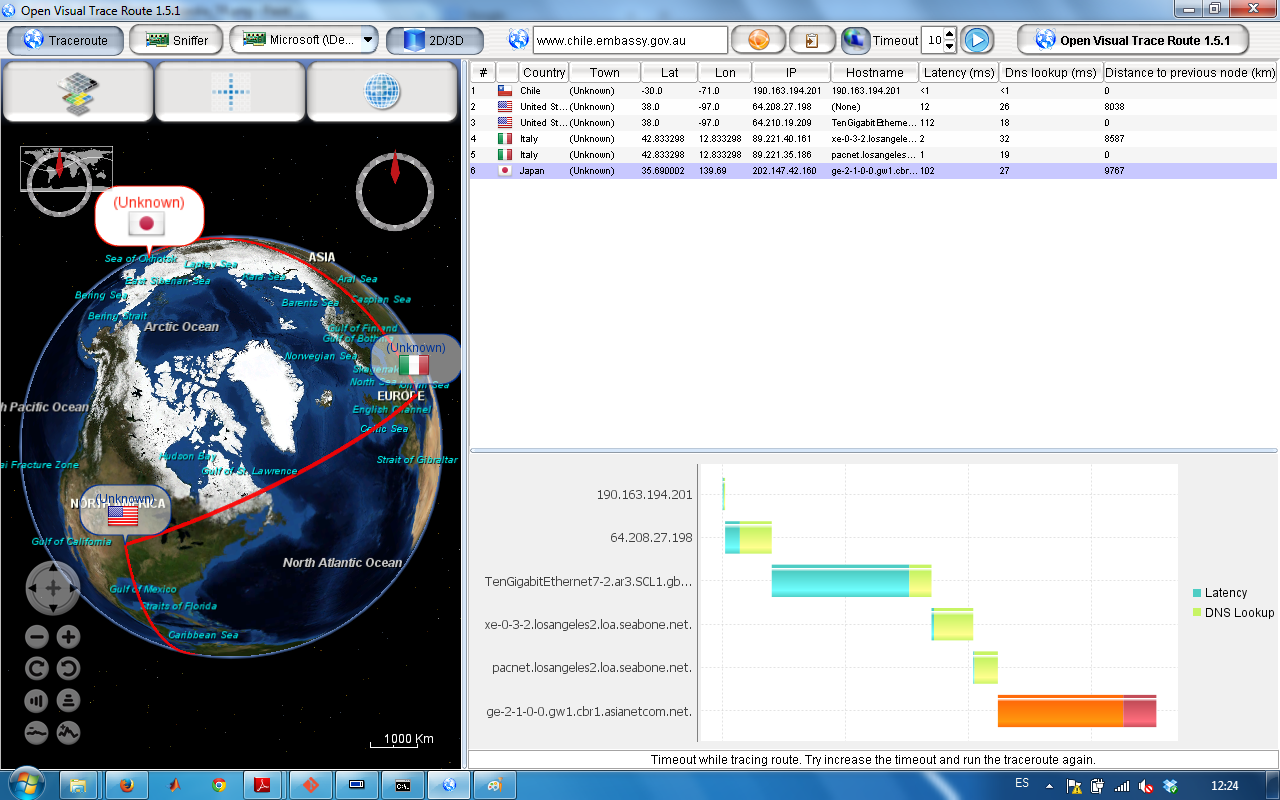
\includegraphics[width=6in]{Redes_chile-embassy_TR.png}
\end{array}$
\end{center}

\end{itemize}
\end{document}
